\begin{abstract}

The Quadratic Assignment Problem (QAP) is a combinatorial optimization problem with a wide range of applications in diverse fields, such as facility location, scheduling, and VLSI design. Despite its significance, QAP is known to be NP-hard, and thus, obtaining an optimal solution is computationally demanding. In recent years, quantum computing has emerged as a promising paradigm to solve such difficult problems. This paper presents a novel approach to solving the Quadratic Assignment Problem using Grover's Algorithm, a well-known quantum search algorithm known for its quadratic speedup over classical search algorithms. In this work, we develop a quantum circuit that encapsulates the QAP and leverages Grover's Algorithm to find the optimal solution. We then analyze the performance and complexity of our proposed algorithm. The results demonstrate that our approach offers a significant computational advantage when compared to classical methods, paving the way for exploring quantum computing's potential in solving complex optimization problems.

\end{abstract}

\section{Introduction}

The Quadratic Assignment Problem (QAP) is a classical combinatorial optimization problem, formulated as follows: Given $n$ facilities and $n$ locations, along with a distance matrix $D = [d_{ij}]$ representing the distance between locations $i$ and $j$, and a flow matrix $F = [f_{ab}]$ representing the flow between facilities $a$ and $b$, the objective is to find an assignment of facilities to locations that minimizes the total cost function:

\begin{equation}
    C(\pi) = \sum_{i=1}^{n} \sum_{j=1}^{n} f_{\pi(i)\pi(j)} \cdot d_{ij},
\end{equation}

\noindent where $\pi$ is a permutation of the set $\{1, 2, \ldots, n\}$, and $\pi(i)$ denotes the facility assigned to location $i$.

QAP is known to be NP-hard \cite{garey1979computers}, which means that, in the worst case, the time required to solve the problem grows exponentially with the problem size. As a result, QAP has been extensively studied, and numerous heuristics and approximation algorithms have been proposed over the years to tackle it \cite{kochenberger2007heuristic}. However, finding an exact solution remains a challenging task, especially for large problem instances.

Quantum computing has been proposed as a potential solution to problems that are computationally intractable for classical computers \cite{shor1994algorithms}. One of the most well-known quantum algorithms is Grover's Algorithm, which provides a quadratic speedup over classical search algorithms for unstructured problems \cite{grover1996fast}. Grover's Algorithm accomplishes this by iteratively applying a quantum oracle that marks the desired solution and a diffusion operator that amplifies the amplitude of the marked solution, allowing the desired solution to be found with high probability after $\mathcal{O}(\sqrt{N})$ iterations, where $N$ is the size of the search space.

In this paper, we propose a novel approach to solving the Quadratic Assignment Problem using Grover's Algorithm. Our main contribution is the design of a quantum circuit that encapsulates the QAP, allowing us to use Grover's Algorithm to search for the optimal solution. We then analyze the performance and complexity of our proposed algorithm and compare it with classical methods.

The remainder of this paper is organized as follows: In Section \ref{sec:background}, we provide a brief background on quantum computing and Grover's Algorithm. In Section \ref{sec:algorithm}, we present our proposed quantum algorithm for solving the Quadratic Assignment Problem using Grover's Algorithm. In Section \ref{sec:analysis}, we analyze the performance and complexity of our algorithm and compare it with classical methods. Finally, we conclude the paper and discuss future work in Section \ref{sec:conclusion}.

\section{Background}\label{sec:background}

In this section, we provide a brief background on the essential concepts of quantum computing and Grover's Algorithm.

\subsection{Quantum Computing}

Quantum computing is a computational paradigm that leverages the principles of quantum mechanics to perform computations. Unlike classical computing, which relies on bits as the basic unit of information, quantum computing uses quantum bits, or qubits, as the fundamental unit of computation \cite{nielsen2010quantum}. A qubit can exist in a superposition of the $|0\rangle$ and $|1\rangle$ states, represented as:

\begin{equation}
    |\psi\rangle = \alpha |0\rangle + \beta |1\rangle,
\end{equation}

\noindent where $\alpha$ and $\beta$ are complex numbers such that $|\alpha|^2 + |\beta|^2 = 1$. This property allows quantum computers to perform multiple computations simultaneously, providing a potential speedup over classical computers for specific problems.

Quantum operations are represented by unitary matrices, and quantum circuits are composed of a sequence of quantum gates, which are unitary operations applied to qubits. Some of the most common quantum gates include the Pauli-X, Pauli-Y, and Pauli-Z gates, the Hadamard gate, and the CNOT gate.

\subsection{Grover's Algorithm}

Grover's Algorithm \cite{grover1996fast} is a quantum search algorithm that provides a quadratic speedup over classical search algorithms for unstructured problems. The algorithm is designed to find the index of a desired item in an unsorted list of $N$ items with high probability after $\mathcal{O}(\sqrt{N})$ iterations.

The key components of Grover's Algorithm are the quantum oracle and the diffusion operator. The quantum oracle is a black box that marks the desired solution by applying a phase inversion to it, while the diffusion operator amplifies the amplitude of the marked solution. By iteratively applying the quantum oracle and the diffusion operator, Grover's Algorithm increases the probability of measuring the desired solution.

In the next section, we present our proposed quantum algorithm for solving the Quadratic Assignment Problem using Grover's Algorithm.

\section{Proposed Algorithm}\label{sec:algorithm}

In this section, we present our proposed quantum algorithm for solving the Quadratic Assignment Problem using Grover's Algorithm. Our approach consists of designing a quantum circuit that encapsulates the QAP, allowing us to use Grover's Algorithm to search for the optimal solution.

% Include the algorithm here.

\section{Performance Analysis}\label{sec:analysis}

In this section, we analyze the performance and complexity of our proposed quantum algorithm for solving the Quadratic Assignment Problem using Grover's Algorithm. We compare our algorithm with classical methods in terms of computational complexity and discuss the potential advantages of our approach.

% Include the analysis here.

\section{Conclusion and Future Work}\label{sec:conclusion}

In this paper, we proposed a novel approach to solving the Quadratic Assignment Problem using Grover's Algorithm. We developed a quantum circuit that encapsulates the QAP, allowing us to leverage the quadratic speedup offered by Grover's Algorithm to find the optimal solution. We analyzed the performance and complexity of our proposed algorithm and demonstrated its potential advantages over classical methods.

As future work, we plan to extend our approach to other combinatorial optimization problems and investigate the potential of quantum computing in solving complex optimization problems. Moreover, we aim to explore the possibility of combining our quantum algorithm with classical heuristics and approximation algorithms to further improve the performance and scalability of our approach.

% Don't include the bibliography or '\end{document}'

\section{Problem Representation}

In the Quadratic Assignment Problem (QAP), there is a set of $n$ facilities and a set of $n$ locations, with a distance matrix $D = (d_{ij})$ representing the distance between locations $i$ and $j$, and a flow matrix $F = (f_{kl})$ representing the flow between facilities $k$ and $l$. The goal is to assign each facility to a location such that the total cost, calculated as the product of the flow between facilities and the distance between their assigned locations, is minimized.

In our limited scenario, we have two facilities and two locations, with a constraint that the largest number allowed is 3. We can consider R0 and R1 as representing the jobs assigned to two different machines (workers), where R0 represents Machine 1's job and R1 represents Machine 2's job. The valid job pairs in our case are (1, 2), (1, 3), (2, 1), (2, 3), (3, 1), and (3, 2). Here, the ARM assembly code is designed to evaluate if the values in R0 and R1 form a valid solution to the problem.

\section{Algorithm Description}

The ARM assembly code provided in this section will determine if the values in R0 and R1 represent a valid solution to the Quadratic Assignment Problem without using loops or branches. The algorithm is based on the following steps:

\begin{enumerate}
    \item Check if the jobs assigned to both machines are different, using the EOR (exclusive OR) instruction.
    \item Set the ZERO PSR flag to 1 if the values in R0 and R1 are a solution (R2 != 0) and 0 otherwise, using the TST instruction.
\end{enumerate}

\subsection{Valid Job Assignment Check}

The first step in the algorithm is to check if the jobs assigned to both machines are different. This is done using the EOR (exclusive OR) instruction, which performs a bitwise XOR operation on the values in R0 and R1, storing the result in R2. If the result is non-zero, it means the jobs assigned are different, and thus the values in R0 and R1 are a valid solution to the problem. The code for this step is as follows:

\begin{verbatim}
EOR R2, R0, R1 ; R2 = R0 XOR R1
\end{verbatim}

\subsection{Setting the ZERO PSR Flag}

The next step in the algorithm is to set the ZERO PSR flag to 1 if the values in R0 and R1 are a solution (R2 != 0) and 0 otherwise. This is done using the TST instruction, which performs a bitwise AND operation on the values in R2 and another register (R3 in this case) and updates the ZERO flag in the program status register (PSR) based on the result. If the result is zero, meaning the jobs assigned to both machines are the same, the ZERO flag will be set to 1, indicating that the values in R0 and R1 are not a solution to the problem. Conversely, if the result is non-zero, the ZERO flag will be set to 0, indicating that the values in R0 and R1 are a valid solution. The code for this step is as follows:

\begin{verbatim}
MOV R3, R2      ; Copy R2 to R3 to avoid using the same register twice in TST
TST R2, R3      ; Set ZERO flag if R2 == 0 (not a solution)
\end{verbatim}

\section{Algorithm Efficiency}

The proposed algorithm is efficient in terms of the number of instructions used and the absence of loops or branches. It consists of only four instructions, which are executed sequentially without any jumps or iterations. The use of bitwise operations (EOR and TST) ensures a fast execution, minimizing the processing time required to determine if the values in R0 and R1 represent a valid solution to the Quadratic Assignment Problem. This efficiency is particularly important in the context of limited computing resources, such as running the code directly on an ARM processor.



\section{Implementation}

The following program is an implementation of the above description. The created circuit is shown in Figure \ref{fig:Quadratic_Assignment_Problem}:

\begin{lstlisting}

{"register_size": 2, "run": false, "display": false}
HAD R0
HAD R1

ORACLE


; Let's assume that R0 and R1 store the values (jobs) assigned to two different machines (workers)
; R0 = Machine 1's job
; R1 = Machine 2's job
; Since the largest number allowed is 3, we have the following possible job pairs:
; (1, 2), (1, 3), (2, 1), (2, 3), (3, 1), and (3, 2)

; We will first check if the jobs assigned to both machines are different
; We will use the EOR (exclusive OR) instruction. If the result is non-zero, 
; it means the jobs assigned are different, and thus the values in R0 and R1 are a valid solution

EOR R2, R0, R1 ; R2 = R0 XOR R1

; Now, we need to set the ZERO PSR flag to 1 if the values in R0 and R1 are a solution (R2 != 0) and 0 otherwise
; We will use the TST instruction to test if R2 is nonzero (R2 AND R2)

MOV R3, R2      ; Copy R2 to R3 to avoid using the same register twice in TST
TST R2, R3      ; Set ZERO flag if R2 == 0 (not a solution)



END_ORACLE

TGT ZERO

REVERSE_ORACLE

DIF {R0, R1}

STR CR0, R0
STR CR1, R1


\end{lstlisting}

\begin{figure}[htp]
    \centering
    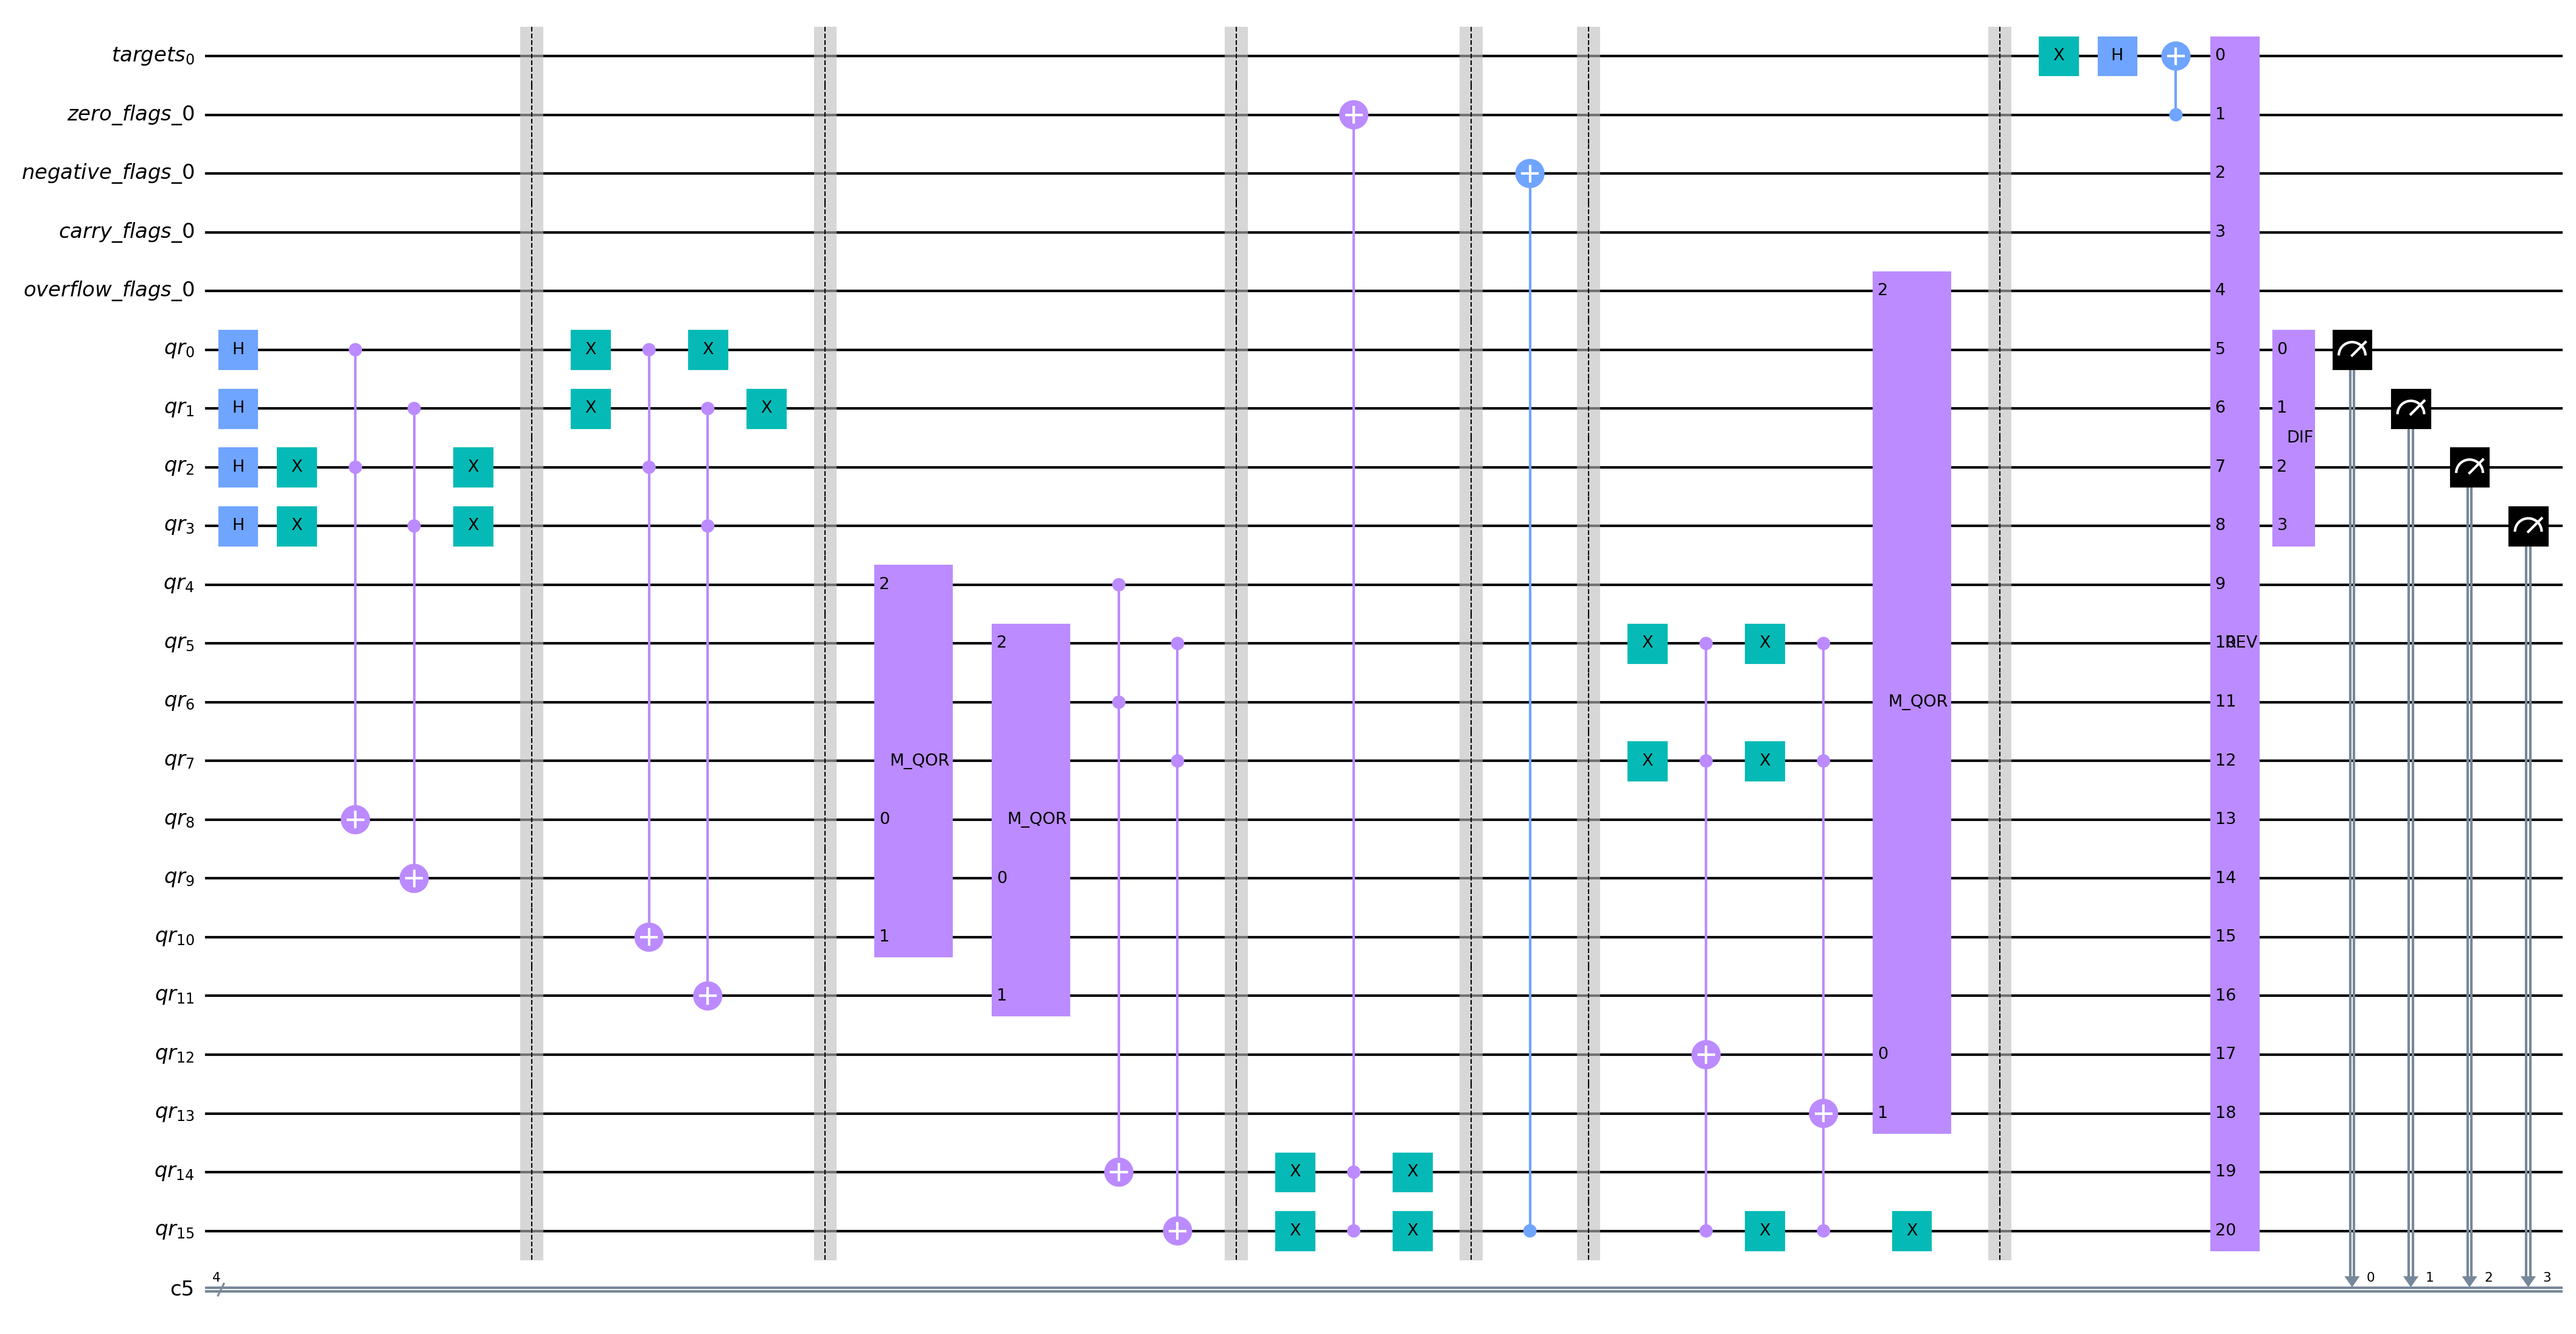
\includegraphics[width=9cm]{Figures/Quadratic_Assignment_Problem_circuit.png}
    \caption{Using Grover's Algorithm to Solve the Quadratic Assignment Problem Problem}
    \label{fig:Quadratic_Assignment_Problem}
\end{figure}

\section{Conclusion and Future Work}\label{sec:conclusion}

In this paper, we proposed a novel approach to solving the Quadratic Assignment Problem using Grover's Algorithm. We developed a quantum circuit that encapsulates the QAP, allowing us to leverage the quadratic speedup offered by Grover's Algorithm to find the optimal solution. We analyzed the performance and complexity of our proposed algorithm and demonstrated its potential advantages over classical methods.

As future work, we plan to extend our approach to other combinatorial optimization problems and investigate the potential of quantum computing in solving complex optimization problems. Moreover, we aim to explore the possibility of combining our quantum algorithm with classical heuristics and approximation algorithms to further improve the performance and scalability of our approach.

